\chapter{\textbf{Аналитический раздел}}

В данном разделе рассматривается предметная область, проводится постановка задачи, производится анализ подходов к реализации различных этапов.

\section{Постановка задачи}

Классификация документов является одной из задач информационного поиска, которая заключается в определении документа к одной из нескольких категорий на основе его содержания.

Задачу классификации типа удостоверения личности на изображении, рассматриваемую в данной работе, можно сформулировать следующим образом.

Существует множество документов, удостоверяющих личность, а также множество заранее известных классов документов. Изображение удостоверения личности Q должно быть отнесено к одному из классов $C=C_i, i \in [0, N]$ с определенной вероятностью.

Данное программное обеспечение предоставляет возможность классификации документов следующих типов. 
\begin{enumerate}
\item[1.] Паспорт гражданина Российской Федерации.
\begin{enumerate}
\item Первая страница -- когда и кем выдан.
\item Вторая страница -- фотография и личные данные
\item Третья страница -- прописка.
\end{enumerate}
\item[2.] Водительское удостоверение.
\begin{enumerate}
\item Образец №1 -- ламинированное бумажное с 1995 по 2011.
\item Образец №2 -- пластиковое с 1995 по 2011.
\item Образец №3 -- удостоверение нового образца.
\end{enumerate}
\item[3.] Загранпаспорт гражданина Российской Федерации.
\item[4.] Шенгенская виза.
\begin{enumerate}
\item Франция.
\item Германия.
\item Италия.
\item Испания.
\end{enumerate}
\end{enumerate}

Классификатор получает входные данные: фотографию документа. На выходе классификатор сообщает, что он получил (паспорт, водительское удостоверение и так далее).

\section{Существующие решения}

Необходимо рассмотреть существующие решения и целесообразность создания нового. На рынке представлено множество разнообразных систем, занимающихся распознаванием документов, как платных, так и бесплатных.

\begin{enumerate}
\item[1.] \textbf{Smart ID Engine} \cite{smartengine}.

\item[2.] \textbf{ABBYY} \cite{abbyy}.

\item[3.] \textbf{IRIS} \cite{iris}.

\item[4.] \textbf{Jumio} \cite{jumio}.

\item[5.] \textbf{Idmatch} \cite{idmatch}.
\end{enumerate}

Проведем сравнение данных решений, представлено в таблице \ref{table:deccompare}.

\begin{table}[H]
\caption{Сравнение существующих решений. }
\begin{tabular}{|p{1.5cm}|p{3.5cm}|p{3cm}|p{2cm}|p{2.5cm}|p{2.3cm}|}
\hline
 & Распознавамые документы & Распознавае- мые языки & Платфор- мы & Доступ- ность & Дополни- тельно \\ \hline
Smart ID Engine & Международные документы (паспорта, визы, водительские права) & Все основные & \begin{tabular}[c]{@{}l@{}}Android \\ iOS \\ Windows \\ MacOSX\end{tabular} & Платное & Сильно ориентируется на машинно-читаемую строку \\ \hline

ABBYY & Международные документы (паспорта, визы, водительские права) & Все основные & \begin{tabular}[c]{@{}l@{}}Android\\ iOS \\ Windows \\ Linux\end{tabular} & Платное & \\ \hline

IRIS & Документы США, международные паспорта и ID-карты & Нет поддержки русского & \begin{tabular}[c]{@{}l@{}}Windows \\ MacOSX\end{tabular} & Платное & \\ \hline

Jumio & Документы Европы и США & Нет поддержки русского & \begin{tabular}[c]{@{}l@{}}Android\\ iOS\end{tabular} & Платное & \\ \hline
Idmatch & Id-карты Кыргызской Республики & Киргизский и русский языки & Нет готового ПО & Бесплатное & \\ \hline
\end{tabular}
\label{table:deccompare}
\end{table}

\textbf{Вывод по таблице}

IRIS, Jumio, Idmatch -- не идентифицируют необходимые документы. ABBYY -- решение подходит только для мобильных устройств. Smart ID Engine -- плохо идентифицирует документы при закрытии машинно-читаемой строки. Необходимо создать собственное решение.

\section{Классификация документов по визуальным признакам}

Далее необходимо рассмотреть этапы обработки изображения, а именно методы классификации по визуальным и текстовым признакам.

Для начала, рассмотрим способы классификации документов по визуальным признакам.

Оптимальным методом классификации являются \textbf{нейронные сети}. 

Существует множество архитектур нейронных сетей, необходимо проанализировать и сравнить их.

\subsection{Выбор модели нейронной сети}

Задача классификации изображений является популярной и хорошо изученной. Выбор алгоритма классификации будет производится на базе результатов международного соревнования ILSVRC \cite{ILSVRC} (ImageNet Large Scale Visual Recognition Challenge). Соревнование оценивает алгоритмы обнаружения объектов и классификации изображений. Его целью является выявление самых лучших с точки зрения точности и скорости алгоритмов обнаружения и классификации. Оценка алгоритмов производится с помощью выборки данных ImageNet \cite{imagenet}. Эта выборка представляет из себя большую визуальную базу данных, содержащую более 14 миллионов изображений, которые в свою очередь разбиваются на 21841 категорию.

Начиная с 2012 года данное соревнованию выигрывают сверточные нейронные сети (Convolutional Neural Networks), а именно AlexNet \cite{alexnet}, ZFNet \cite{zfnet}, VGGNet \cite{vggnet}, GoogLeNet \cite{googlenet}, ResNet \cite{resnet}, TrimpsNet (Не было никакого нового научного вклада, который оправдывал бы подготовку статьи, и по этой причине авторы TrimpsNet только поделились результатами) и SENet \cite{senet}. С 2015 года CNN превзошли человеческие показатели -- 5.1\% \cite{human}. 

\begin{enumerate}
\item[1.] \textbf{AlexNet}.

AlexNet была первой свёрточной нейронной сетью, выигравшей соревнование по классификации ImageNet в 2012 году. Архитектура AlexNet состоит из пяти свёрточных слоев, между которыми располагаются пулинг слои и слои нормализации, три полносвязанных слоя завершают нейронную сеть.

На схеме архитектуры все выходные изображения разделены на две одинаковые части -- это связано с тем, что нейронная сеть обучается на старом GTX580, который имел всего 3 ГБ видеопамяти. Для обработки использовались две видеокарты, чтобы параллельно выполнять операции над двумя частями изображения.

\item[2.] \textbf{ZFnet}.

В 2013 году нейросеть ZFnet смогла достичь результата 11.7\% -- архитектура AlexNet использовалась в качестве основы, но с изменёнными параметрами и слоями. 

\item[3.] \textbf{VGGnet}.

Появилась в 2014 году. Основная идея -- использовать вместо больших сверток (11x11 и 5x5) маленькие свертки (3x3). С маленькими фильтрами мы получим не так много параметров, но при этом сможем гораздо эффективнее обрабатывать их.

\item[4.] \textbf{GoogleNet}.

GoogleNet или Inception-v1 -- ещё более глубокая архитектура с 22 слоями. Целью Google было разработать нейросеть с наибольшей вычислительной эффективностью. Для этого они придумали так называемый модуль Inception --- вся архитектура состоит из множества модулей, следующих друг за другом.

\item[5.] \textbf{ResNet}.

ResNet -- это сокращенное название для Residual Network (дословно -- «остаточная сеть»). Решает проблему деградации (простая сеть увеличивает частоту ошибок по мере того, как сеть углубляется), и после использования остатка, когда сеть углубляется, частота ошибок все еще может уменьшаться.

\item[6.] \textbf{SENet}.

Squeeze-and-Excitation Networks (SENets) представляют собой специальный блок для свёрточной нейронной сети, который улучшает взаимозависимости каналов практически без дополнительных вычислений. Основная идея -- добавить параметры к каждому каналу свёрточного блока, чтобы сеть могла адаптивно регулировать вес каждой карты признаков. 

\end{enumerate}

В ImageNet основными метриками ошибок являются: top-1 и top-5, где частота ошибок top-5 -- это доля тестовых изображений, для которых правильная метка не входит в число пяти меток, которые модель считает наиболее вероятными.

Результаты сравнения моделей представлены в таблице \ref{table:cnncompare}.

\begin{table}[H]
\caption{Сравнение моделей сверточных нейронных сетей. }
\begin{tabular}{|p{2.5cm}|p{1.5cm}|p{2cm}|p{5cm}|p{4cm}|}
\hline
Название сети \cite{cnn} & Год & Ошибка Top-5 & Количество обучаемых параметров \cite{numparams} & Требуемое оборудование \cite{gpu} \\ \hline
AlexNet    & 2012 & 16.4 \% & 60 миллионов & 2 GPU \\ \hline
ZFNet     & 2013 & 11.7 \%  & 60 миллионов  & 1 GPU \\ \hline
VGGNet    & 2014 & 7.3 \%  & 138 миллионов & 4 GPU \\ \hline
GoogleNet   & 2014 & 6.7 \%  & 4 миллиона & CPU \\ \hline
ResNet    & 2015 & 3.5 \%  & 25.6 или 1.7 миллиона & 2 GPU \\ \hline
TrimpsNet   & 2016 & 2.99 \%  & & \\ \hline
SENet     & 2017 & 2.25 \%  & 27.5 миллионов & 8 GPU \\ \hline
\end{tabular}
\label{table:cnncompare}
\end{table}

\textbf{Вывод по таблице}

В соответствии с результатами ILSVRC последних лет, можно отметить, что наилучшей точностью классификации объектов на сегодняшний день обладает свёрточная нейронная сеть SENet. Однако этот алгоритм является очень требовательным к вычислительным ресурсам.

Принято компромиссное решение -- использовать модель нейронной сети GoogleNet, так как она дает хорошие показатели точности и не требует мощные вычислительные ресурсы.

\section{Обзор и анализ методов распознавания и классификации текстовой информации}

Второй составляющей метода является распознавание и классификация текстовой информации в документе.

Таким образом, процесс делится на три связанных между собой этапа:

\begin{itemize}
\item этап выделения текстовой информации из изображения;
\item этап преобразования текста в вектор признаков, в процессе которого определяется наиболее полное и информативное представление текста в виде числового вектора;
\item этап классификации, в процессе которого проверяется гипотеза принадлежности изображения классу изображений объекта на основании наблюдения (вектора признаков).
\end{itemize}

\subsection{Оптическое распознавание символов}

Преобразование графического изображения в текст выполянетя специальными программами распознавания текста (Optical Character Recognition - OCR).

Основной принцип автоматического распознавания образов заключается в обучении машины распознавать все возможные эталонные образцы и сравнивать их с идентифицированными объектами. В системах распознавания это буквы, цифры и знаки препинания. Обучение осуществляется путем показа машине образцов символов различных классов. На основе этих образцов машина генерирует прототип описания каждого класса объекта. Затем в процессе распознавания неизвестные символы сравниваются с заранее полученными образцами (выборкой) и определяется класс, с которым обнаружено больше всего совпадений.

Системы оптического распознавания текста -- OCR-системы технология, которая позволяет преобразовывать различные типы документов, такие как отсканированные документы, PDF-файлы или фото с цифровой камеры, в редактируемые форматы с возможностью поиска \cite{ocr}. 

OCR -- это одно из направлений компьютерного зрения. 

Современные системы оптического распознавания можно разделить на коммерческие и свободно распространяемые системы с открытыми исходными кодами.

Для сравнения интерес представляют обе системы, как коммерческие, ориентированные на высокое качество распознавания, так и открытые системы, ориентированные на доступность и гибкость конфигурации. Поскольку целью данной работы является работа с документами на языках: русском, английском, испанском, французском, итальянском, немецком, интерес представляют системы, поддерживающей распознавание данных языков.

\textbf{ABBYY FineReader} \cite{finereader} -- это программное обеспечение оптического распознавания символов (OCR). Поддерживает распознавание текста на 190 языках. OCR или распознавание текста, использует интеллектуальные алгоритмы для преобразования изображений в редактируемый текст с сохранением исходного макета и формата исходного документа. Является признанным лидером на рынке. Распространяется на коммерческой основе.

\textbf{IRIS Readiris} \cite{readiris} -- это программа для преобразования документов в различные форматы. Распознает более 130 языков, включая русский, принимает файлы и сохраняет результаты во всех возможных форматах. Программное обеспечение платное. 

\textbf{Cuneiform} \cite{cuneiform} -- свободно распространяемая открытая система оптического распознавания текстов российской компании Cognitive Technologies. CuneiForm позиционируется как система преобразования электронных копий бумажных документов и графических файлов в редактируемый вид, способная сохранять структуру и тип шрифта исходного документа в автоматическом или полуавтоматическом режиме. Система включает в себя две программы для одиночной и пакетной обработки электронных документов. Поддерживает все необходимые нам языки: английский, русский, испанский, итальянский, французский, немецкий. Кроме того, поддерживается сочетание русского и английского языка. 

\textbf{Tesseract} \cite{tesseract} -- свободная компьютерная программа для распознавания текстов, разрабатывавшаяся Hewlett-Packard, а затем Google купил её и открыл исходный код под лицензией Apache 2.0 для продолжения разработки. Сегодня Tesseract считается одним из самых мощных решений с открытым исходным кодом для распознавания данных отсканированных документов. Tesseract поддерживает более 100 различных языков, что делает его универсальным и широко используемым решением во всём мире. Многие технологические компании создают комплексные интеллектуальные решения для обработки данных, в основе которых лежит Тессеракт.

\textbf{OCRFeeder} \cite{ocrfeeder} -- программа, предоставляющая графический интерфейс пользователя для систем оптического распознавания символов CuneiForm, Tesseract, GOCR и Ocrad. OCRFeeder является свободно распространяемой программой для операционной системы Linux.

Выбор OCR систем основывался на сравнительном анализе их результатов по трем типам данных (среднее качество, высокое качество и очень высокое качество) \cite{textocr}. Примеры изображений приведены на рисунках \ref{img:quality1}, \ref{img:quality2}, \ref{img:quality3}.

\begin{figure}[H]
	\centering
	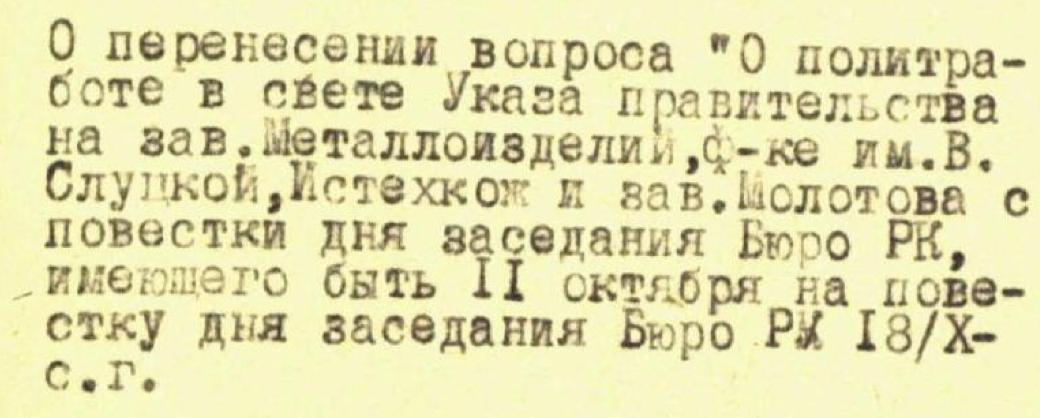
\includegraphics[scale=0.7]{quality1}
	\caption{Среднее качество. }
	\label{img:quality1}
\end{figure}

\begin{figure}[H]
	\centering
	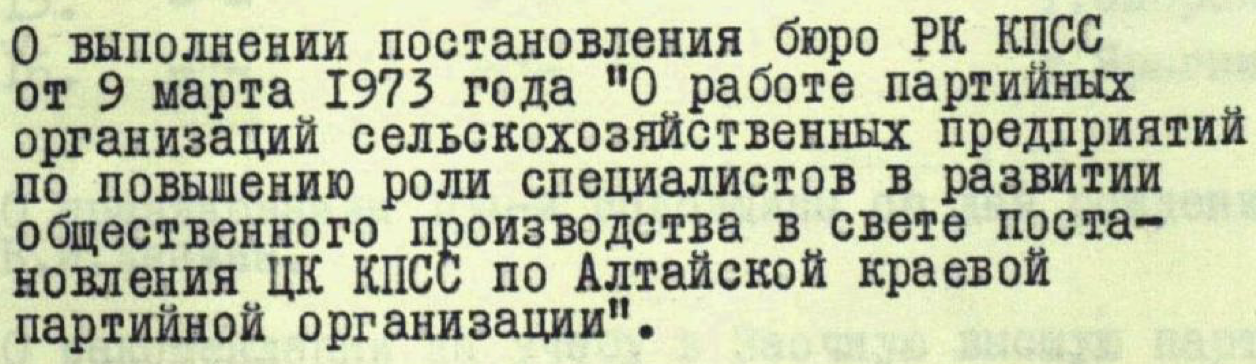
\includegraphics[scale=0.7]{quality2}
	\caption{Высокое качество. }
	\label{img:quality2}
\end{figure}

\begin{figure}[H]
	\centering
	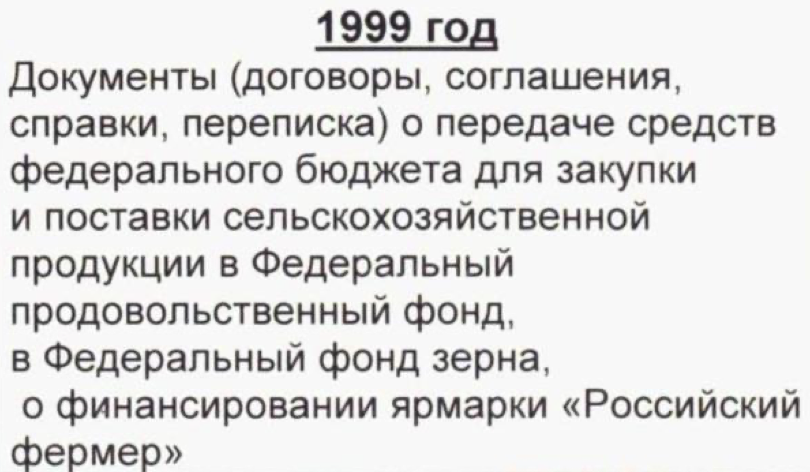
\includegraphics[scale=0.7]{quality3}
	\caption{Очень высокое качество. }
	\label{img:quality3}
\end{figure}

Качество результатов распознавания представлено в таблице \ref{table:comparetext}.

\begin{table}[H]
\caption{Сравнение качества распознавания текста.}
\begin{tabular}{|p{3cm}|p{3cm}|p{3cm}|p{3cm}|p{3cm}|}
\hline
& Качество распознавания документов среднего качества & Качество распознавания документов высокого качества & Качество распознавания документов очень высокого качества & Доступность \\ \hline
ABBYY FineReader & 76,8\% & 90,55\% & 99,25\% & коммерческое\\ \hline
IRIS Readiris & 22,01\% & 68,34\% & 94,40\% & коммерческое \\ \hline
Cuneiform & 0\% & 30,28\% & 90,20\% & open-source \\ \hline
Tesseract & 36,06\% & 74,68\% & 94,13\% & open-source \\ \hline
\end{tabular}
\label{table:comparetext}
\end{table}

\textbf{Вывод по таблице}

Результаты сравнительного анализа показывают, что коммерческая система <<Abby Finereader>> достигает максимального уровня качества. В свободно распространяемых системах лучшим является -- Tesseract.

\subsection{Индексация текста}

Индексация документов -- это получение вектора признаков для текста, состоит из двух этапов: получение термов и взвешивание термов.

Модели перевода текста в векторное пространство \cite{indexdocs}.
\begin{enumerate}
\item[1.] \textbf{Мешок слов}.
В данной модели порядок слов не имеет значения, все документы представлены матрицей, где строка -- это документ, столбец -- слово. Элемент на пересечении строки и столбца -- вес слова в документе.
\item[2.] \textbf{Мешок N-грамм}.
Часто информацию несут не только отдельные слова, но некоторые последовательности. В данной модели учитываются вместо слов последовательности из N слов. Все документы будут также представлены матрицей.
\item[3.] \textbf{Word2vec}.
Для каждого слова находится его векторное представление, которое содержит информацию о контекстных словах. После чего применяется метод кластеризации и в новом виде тексты состоят не из слов, а из номеров кластеров.
\end{enumerate}

Далее необходимо рассмотреть различные функции взвешивания \cite{weightsfunc}.

\begin{enumerate}
\item[1.] \textbf{Частотные векторы}.
Заполняем вектор частотой, с которой слово появляется в документе.

Например, на рисунке \ref{img:freq} представлено, как бы выглядел вектор для текста номер 2.

\begin{figure}[H]
	\centering
	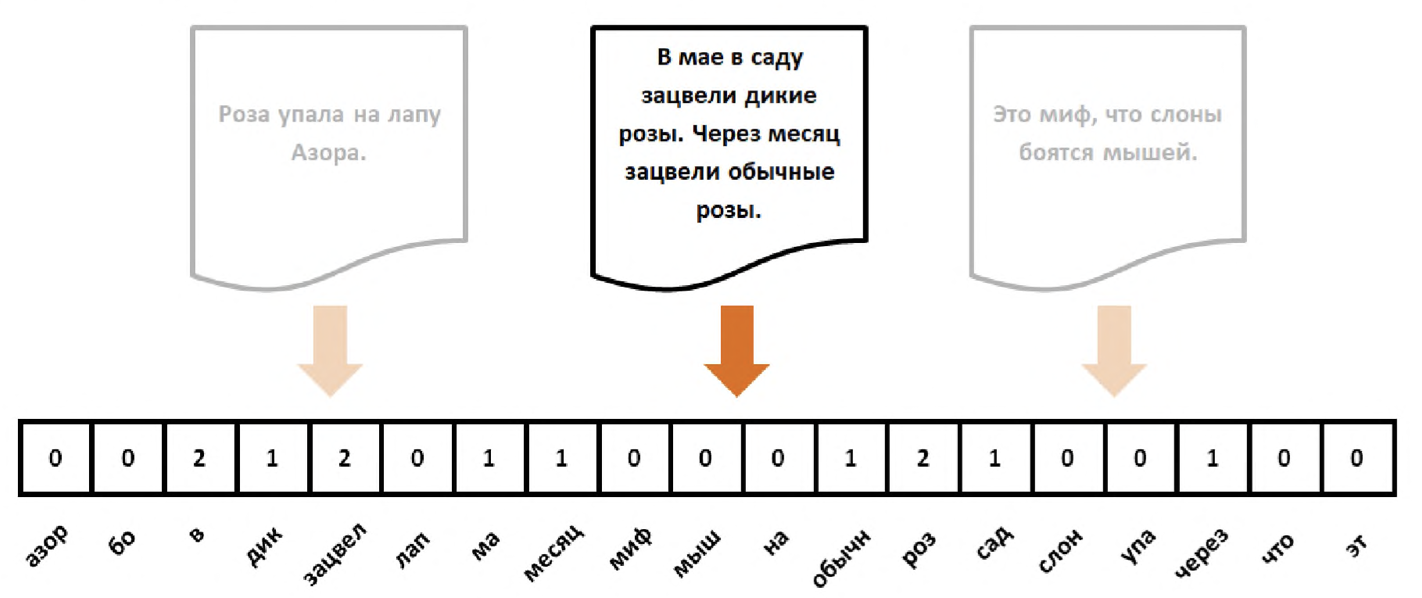
\includegraphics[scale=0.65]{freq}
	\caption{Функция взвешивания, частотные векторы }
	\label{img:freq}
\end{figure}

\item[2.] \textbf{Унитарное кодирование}.
Заполняем вектор значениям 1 или 0, в зависимости от того есть ли слово в документе, или его нет, соответсвенно.

Например, на рисунке \ref{img:uni} представлено, как бы выглядел вектор для текста номер 1.

\begin{figure}[H]
	\centering
	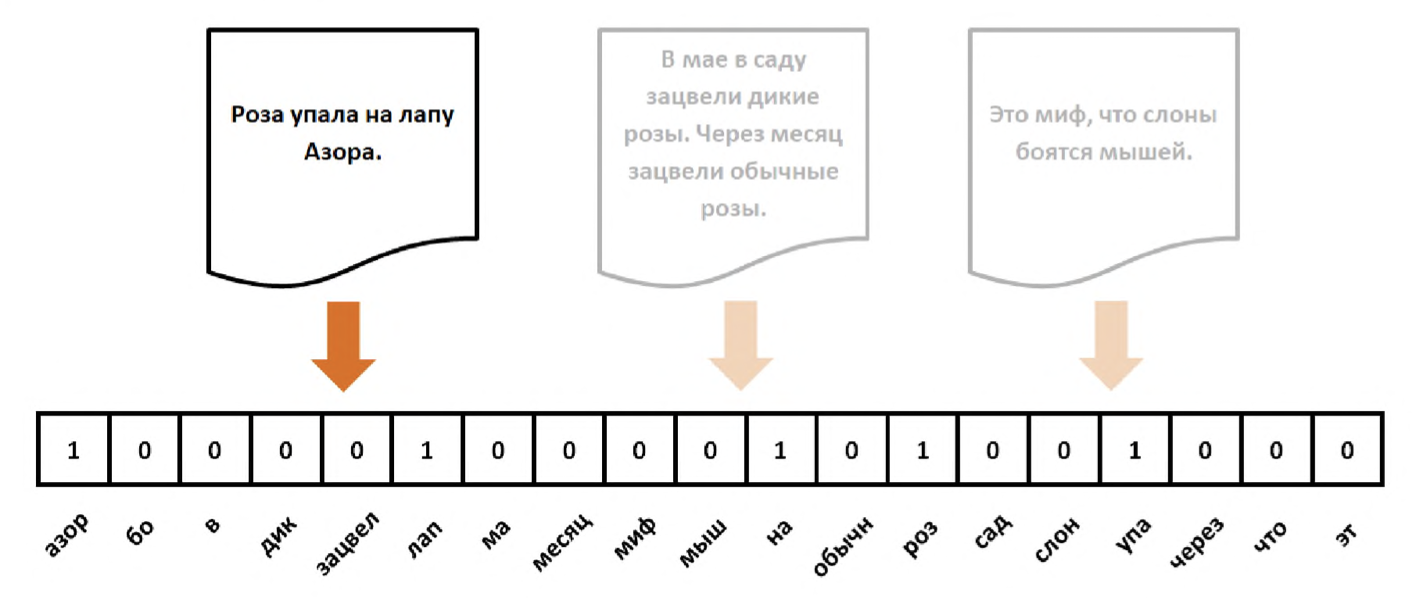
\includegraphics[scale=0.65]{uni}
	\caption{Функция взвешивания, унитарное кодирование }
	\label{img:uni}
\end{figure}

\item[3.] \textbf{Частота слова -- обратная частота документа (TF\_IDF)} \cite{classes}.

TF\_IDF нормализует частоту токенов в документе по отношению к остальной части. Подход подчеркивает термины, которые часто встечаются в пределах данного документа и резко употребляются в других.

Частота термина TF -- оценка важности слова $t$ в пределах одного документа $d$, вычисляется по формуле \ref{eq:tf}.

\begin{equation}
	\centering
	TF = \frac{n_{t,d}}{n_d}
	\label{eq:tf}
\end{equation}

Обратная частота документа IDF -- инверсия частоты, с которой слово $t$ встречается в документах коллекции, вычисляется по формуле \ref{eq:idf}.

\begin{equation}
	\centering
	IDF = \log{\frac{|D|}{D_t}}
	\label{eq:idf}
\end{equation}

Итоговый вес слова в документе относительно всех документов вычисляется по формуле \ref{eq:tfidf}

\begin{equation}
	\centering
	V_{t,d} =TF \cdot IDF
	\label{eq:tfidf}
\end{equation}

Например, на рисунке \ref{img:tfidf} представлено, как бы выглядел вектор для текста номер 3.

\begin{figure}[H]
	\centering
	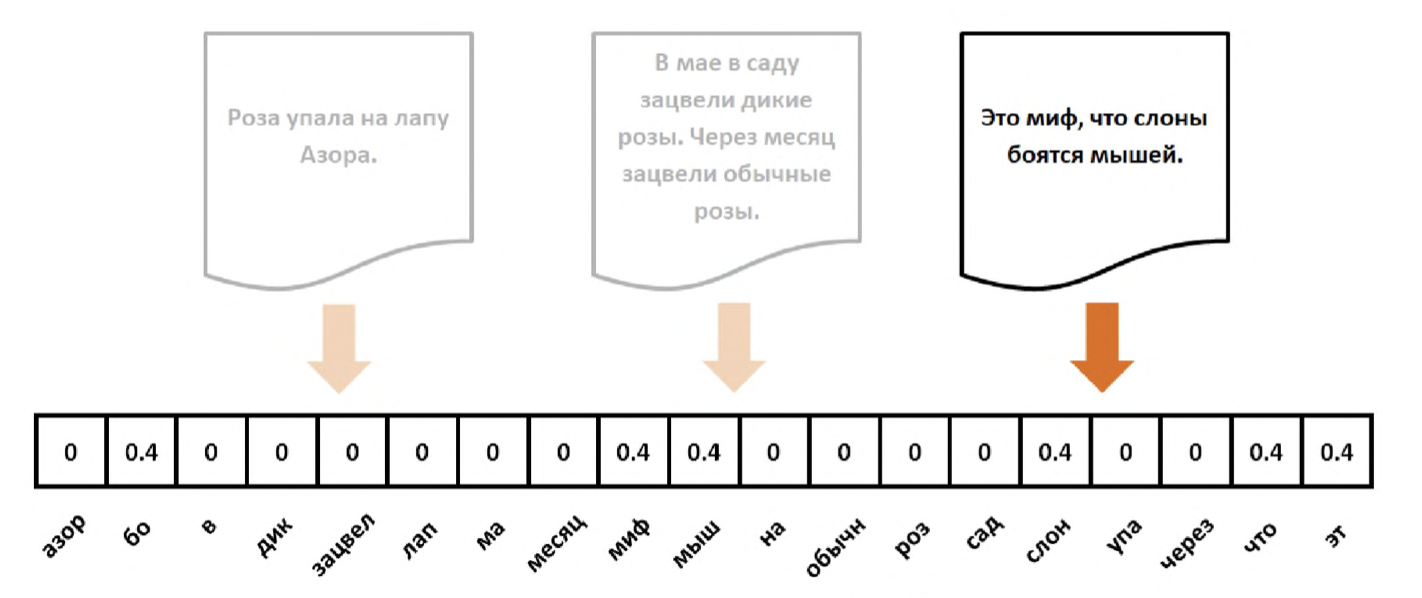
\includegraphics[scale=0.65]{tfidf}
	\caption{Функция взвешивания, TF\_IDF }
	\label{img:tfidf}
\end{figure}
\end{enumerate}

\textbf{Вывод по сравнению методов индексации текста}

В данной работе последовательность слов и их семантика значения не имеет, поэтому было приятно решение использовать модель -- мешок слов. Весовой функцией выбрана -- TF\_IDF, так как в документах встречаются слова, которые появляются только в одном, а значит более важны. А есть слова, которые встречаются во многих и их значимость будет меньше.

\subsection{Методы классификации}

Существует множество методов классификации, которые используют различный математический аппарат и различные подходы при реализации. Однако эффективность этих методов зависит от конкретной решаемой задачи. Несмотря на то, что в течение последнего десятилетия коммерческие компании занимаются проблемой повышения качества машинного обучения, на сегодняшний день не существует методов, которые могли бы однозначно эффективно решить задачу классификации. 

Можно выделить следующие типы методов классификации: вероятностные, метрические, логические, линейные, логическая регрессия \cite{classes}. Необходимо обобщенно описать некоторые из них, указывая преимущества и недостатки каждого из них. 

\begin{enumerate}
\item[1.] \textbf{Метод Байеса}.

Метод Байеса (Naive Bayes, NB) относится к вероятностным методам классификации \cite{baes}. 

Пусть имеется множество классов $C = \{c_0, c_1, ..., c_N\}$ документов. Согласно теореме Байеса вероятность того, что документ принадлежит классу $c$, имеет вид \ref{eq:baies}.

\begin{equation}
	\centering
	P(c|d)=\frac{P(c)P(d|c)}{P(d)}
	\label{eq:baies}
\end{equation}

Вероятность $P(d)$ не требует вычислений ввиду того, что его значение не зависит от класса $c$, а значит, не влияет на нахождение наибольшей вероятности. 

Преимущества метода состоит в следующем: 
\begin{itemize}
\item высокая скорость работы;
\item поддержка инкрементного обучения;
\item простая реализация алгоритма в виде программы,;
\item легкая интерпретируемость результатов работы алгоритма. 
\end{itemize}

Несмотря на приведенные достоинства, метод Байеса имеет так же и минусы в своей реализации. 
\begin{itemize}
\item Относительно низкое качество классификации. 
\item Неспособность учитывать зависимость результата классификации от сочетания признаков являются главными недостатками этого метода.
\end{itemize}

\item[2.] \textbf{Метод k ближайших соседей}.

Метод k ближайших соседей (k Nearest Neighbors, KNN) относится к метрическим методам и считается простейшим классификатором \cite{neighbors}. Суть метода заключается в том, что документу $d$ присваивается тот класс $c$, к которому принадлежит большинство из $k$ ближайших соседей документа, вычисленных с помощью какой-либо метрики расстояния.

Достоинства данного метода: 
\begin{itemize}
\item простая реализация;
\item легкая интерпретируемость.
\item возможность обновления обучающей выборки без переобучения классификатора; 
\item устойчивость алгоритма к аномальным выбросам в исходных данных; 
\item хорошее обучение в случае с линейно неразделимыми выборками.
\end{itemize}

К недостаткам относятся: 
\begin{itemize}
\item недостаточная производительность в реальных задачах, так как число соседей, используемых для классификации, будет достаточно большим; 
\item трудность в наборе подходящих весов и определением, какие признаки необходимы для классификации; 
\item высокая зависимость от выбранной метрики расстояния между примерами;
\item невозможность решения задач большой раз-мерности по количеству классов и документов.
\end{itemize}

\item[3.] \textbf{Метод деревьев решений}.

Метод деревьев решений (Decision Trees, DT) относится к логическим методам классификации \cite{tree}. Дерево решений представляет собой конечный связный граф с множеством вершин, по которому производится классификация документов, описанных набором признаков. В узлах (вершинах) дерева прописаны условия, после проверки которых выполнение алгоритма классификации продолжается по правому или левому поддереву рассматриваемого узла. Процедура повторяется в каждом посещенном узле до тех пор, пока очередной узел не окажется листом. У каждого узла столько ветвлений, сколько значений имеет выбранный признак. 

Метод обладает рядом преимуществ, таких как:
\begin{itemize}
\item простая программная реализация;
\item быстрота обучения;
\item высокая точность прогнозирования. 
\end{itemize}

Однако также присущи и недостатки, такие как:
\begin{itemize}
\item неустойчивость алгоритмов к выбросам;
\item необходим большой объем тренировочных данных для получения точных результатов.
\end{itemize}

\item[4.] \textbf{Метод опорных векторов}.

Метод опорных векторов (Support Vector Machine, SVM) является линейным методом классификации, в настоящее время призван одним из лучших \cite{vectors}. Главным принципом SVM является определение раз- делителя в искомом пространстве, который разделяет классы наилучшим образом.

Преимущества метода: 
\begin{itemize}
\item один из наиболее качественных методов;
\item возможность работы с небольшим набором данных для обучения;
\item сводимость к задаче выпуклой оптимизации, имеющей единственное решение. 
\end{itemize}

Недостатки метода: 
\begin{itemize}
\item сложная интерпретируемость параметров алгоритма;
\item неустойчивость по отношению к выбросам в исходных данных. 
\end{itemize}

\item[5.] \textbf{Логистическая регрессия}.

Одним из ранних применений регрессии к классификации текстов является линейный метод наименьших квадратов (ЛМНК) \cite{linear}.

Преимущества метода:
\begin{itemize}
\item является одним из наиболее качественных;
\item поддерживает инкрементное обучение; 
\item имеет относительно простую программную реализацию алгоритма. 
\end{itemize}

Недостатки метода: 
\begin{itemize}
\item сложная интерпретируемость параметров алгоритма;
\item неустойчивость по отношению к выбросам в исходных данных. 
\end{itemize}

\item[6.] \textbf{Нейронные сети}.
\end{enumerate}

Нейронные сети состоят из набора <<нейронов>>, которые являются преобразователями входных сигналов в выходные \cite{neuron}. Преобразование задается весами сети, которые являются параметрами и могут изменяться. Выходные сигналы вычисляются как функция от входных сигналов. В общем случае нейронная сеть строится как соединение множества нейронов, объединенных в уровни, при этом выходы одного уровня являются входами следующего.
Самая простая нейронная сеть состоит из одного слоя, однако круг решаемых такими сетями задач ограничен. Поэтому на практике часто используют нейронные сети, содержащие большее число слоев.

Преимущества метода:
\begin{itemize}
\item имеет очень высокое качество алгоритма при удачном подборе параметров;
\item является универсальным аппроксиматором непрерывных функций; 
\item поддерживает инкрементное обучение. 
\end{itemize}

Недостатки метода: 
\begin{itemize}
\item вероятность возможной расходимости или медленной сходимости, поскольку для настройки сети используются градиентные методы;
\item необходимость очень большого объема данных для обучения, чтобы достичь высокой точности;
\item низкая скорость обучения;
\item сложная интерпретируемость параметров алгоритма.
\end{itemize}

\textbf{Вывод по анализу методов классификации текстов}

Так как в работе важна точность, при этом без больших нагрузок системы. Для классификации текстовой информации выбран метод опорных векторов.

\section{Вывод}

В данном разделе выполнена постановка задачи работы, проанализированы существующие решения и необходимость создания нового. Были рассмотрены методы классификации документа по визуальным и текстовым признакам. 

Исходя из приведенного сравнительного анализа были выбраны следующие подходы:
\begin{itemize}
\item В качестве модели нейронной сети, для классификации документов по визуальным признакам, была выбрана -- googlenet.
\item Для оптического распознавания текста -- tesseract.
\item Индексация текста -- мешок слов и весовая функция -- частота слова -- обратная частота документа (TF\_IDF).
\item Для классификации текстовой информации -- метод опорных векторов.
\end{itemize}
